%
% PKUMpLtX --- A LaTeX document class for 'Modern Physics Laboratory' in PKU based on `revtex4-2`
%
% Please read `README.md' and the template file before using
% 需要确保 font 选项指定的字体已安装! 具体参见 `README.md' 的说明.
\documentclass[font=default]{mpltx}

% 以下至 \begin{document} 都仅是本文件为了方便额外定义的命令, 写报告时不需要.
\hypersetup{colorlinks=true}% 超链接带颜色
\usepackage{xcolor}
\newcommand{\note}[1]{{\color{gray}#1}}
\NewDocumentCommand{\pkg}{s o m}{%
    \IfBooleanF{#1}{%
        \IfNoValueTF{#2}%
            {\href{https://www.ctan.org/pkg/#3}}%
            {\href{https://www.ctan.org/pkg/#2}}%
    }%
    {\textsf{#3}}%
}
\newcommand*\cs[1]{\texttt{\textbackslash #1}}
\newcommand*\env[1]{\textit{\texttt{#1}}}
\newcommand*\code[1]{\texttt{#1}}
\newcommand*\file[1]{\textbf{\texttt{#1}}}
\makeatletter
\newcommand\releasedate{%
    \href{https://github.com/CastleStar14654/PKUMpLtX/releases/tag/\mpltx@fileversion}%
        {\mpltx@filedate, \mpltx@fileversion}}
\makeatother
% 以上是本文件为了方便额外定义的命令, 写报告时不需要.

\begin{document}

\title{塞曼效应} % 切合报告内容, 简短明确, 可以不同于讲义
\author{郑熔} % 这里 \emailphone 一定要紧跟在 \author 后方
\emailphone{2300011359@stu.pku.edu.cn}{(86)19805861588}
% 如果改用 \email 则仅需要邮箱参数
\affiliation{北京大学物理学院\quad 学号: 2300011359}
% % 可以使用 \zhdate 自动生成中文日期, 如
\date{\zhdate{2025/10/15}}
% % 也可使用 babel 的 \localedate, 如
% \date{\localedate{2020}{12}{1}}
% % 两者均会输出 `2020 年 12 月 1 日'
% 下面的 \date 的参数是为了自动输出正确版本号, 正式报告请替换为上面的两种 \date 之一
% \date{\releasedate}
\begin{abstract}
  塞曼效应是指原子的谱线在外磁场中发生分裂的现象. 
  本实验运用气压扫描式法布里 - 珀罗标准具 (F-P 标准具) , 
  对汞灯 546.1 nm 谱线在无磁场、 4A 励磁电流激发的磁场以及 5A 励磁电流激发的磁场条件下的塞曼谱线进行了测量, 
  并对所得谱线开展了相应分析.
  本实验测量得到了各子谱线与 546.1 nm 谱线的波数差及相对强度,
  将其与理论计算结果对比后,
  对误差来源进行了简要分析.
  此外, 实验还借助光谱数据计算出电子荷质比, 通过与标准值比对发现两者非常接近, 验证了相关理论的正确性.
  % \note{本文档为对 \href{https://github.com/CastleStar14654/PKUMpLtX}{\pkg*{PKUMpLtX}} 的使用示例, 灰色部分为额外针对 \LaTeX{} 模板使用的说明或是一些能提升输出效果的琐碎细节.
    % 也请注意查看源文档 \file{template.tex} 中的注释.}
\end{abstract}
\keywords{塞曼效应, F-P 标准具}

\maketitle

\section{引言}
  1896 年, 荷兰物理学家塞曼 (Pieter Zeeman) 在实验中发现: 
  当钠光源置于足够强的外磁场中时, 其谱线会分裂为若干条子谱线, 
  这一现象后来被命名为  " 塞曼效应" . 塞曼效应分为正常塞曼效应和反常塞曼效应.
  正常塞曼效应是指谱线分裂为三条, 
  裂距一个洛伦兹单位 ($\tilde{L} = \frac{eB}{4\pi mc}$) , 可以用经典理论解释.
  其余为反常塞曼效应, 需要用量子理论解释.
  塞曼效应是继 "法拉第效应" 和 "克尔效应" 之后, 第三个用来说明磁场和电场对光产生影响的例证.
  从塞曼效应的结果中人们可以得到有关能级的数据, 即由分裂后子谱线的个数可以知道能级的 J 值, 从子谱线裂距的大小可以知道 g 因子 \cite{jindaiwulishiyan}.
  \par
  本实验运用气压扫描式法布里 - 珀罗标准具 (F-P 标准具) , 
  对汞灯 546.1 nm 谱线在无磁场、有磁场条件下的塞曼谱线进行了测量, 
  并观察到了谱线的精细结构, 也对所得谱线开展了相应分析.
  本实验测量得到了各子谱线与 546.1 nm 谱线的波数差及相对强度,
  还计算出电子荷质比, 通过与标准值比对发现两者非常接近, 验证了相关理论的正确性, 从而让我们更深刻地了解塞曼效应.

\section{理论}
对于本实验, 汞灯 546.1nm 光谱线对应的跃迁中上、下能级的电子态和光谱项和是$6\mathrm{s}7\mathrm{s}\ ^3\mathrm{S}_1 \rightarrow 6\mathrm{s}6\mathrm{p}\ ^3\mathrm{P}_2$.
根据相关概念, 
$$ 
g = 1 + \frac{J(J + 1) - L(L + 1) + S(S + 1)}{2J(J + 1)} , \Delta E = Mg\frac{eh}{4\pi m}B , M = J, J - 1, \cdots, -J 
$$
对于 $J \to J+1$ 跃迁:
\begin{equation} \label{energy}
\begin{aligned}
&M_J \to M_J \pm 1, & I_\sigma &= \frac{1}{4}(J \pm M_J + 1)(J \pm M_J + 2); \\
&M_J \to M_J, & I_\pi &= (J+1)^2 - M^2
\end{aligned}
\end{equation}
洛伦兹单位  $\tilde{L} = \frac{eB}{4\pi mc} \approx 0.467B$

由此得到理论该实验的塞曼效应的结果\autoref{fig:lilun}, 
其中, 横轴表示各条子谱线相对于无磁场时谱线的位置, 单位为洛伦兹单位 $\tilde{L}$. 
横轴上方的竖线表示 $\pi$ 成分, 横轴下方的竖线表示 $\sigma$ 成分, 线段的长度表示谱线的相对强度, 由\autoref{energy}计算得到. 

\begin{figure}[htbp]
  \centering
  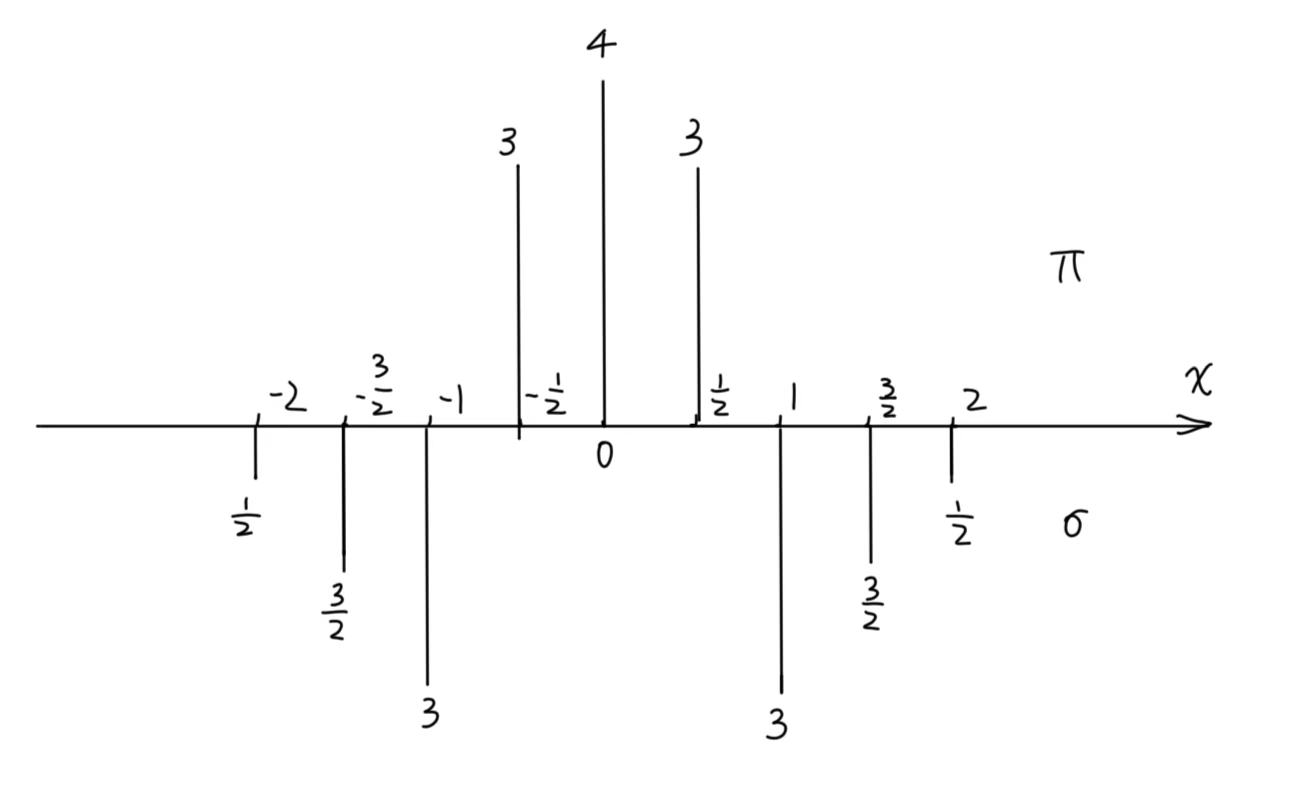
\includegraphics[width=0.85\linewidth]{fig/lilun.jpg}
  \caption{本实验塞曼效应结果示意图}
  \label{fig:lilun}
\end{figure}


\section{实验}
\subsection{实验装置示意}

\begin{figure}[htbp]
  \centering
  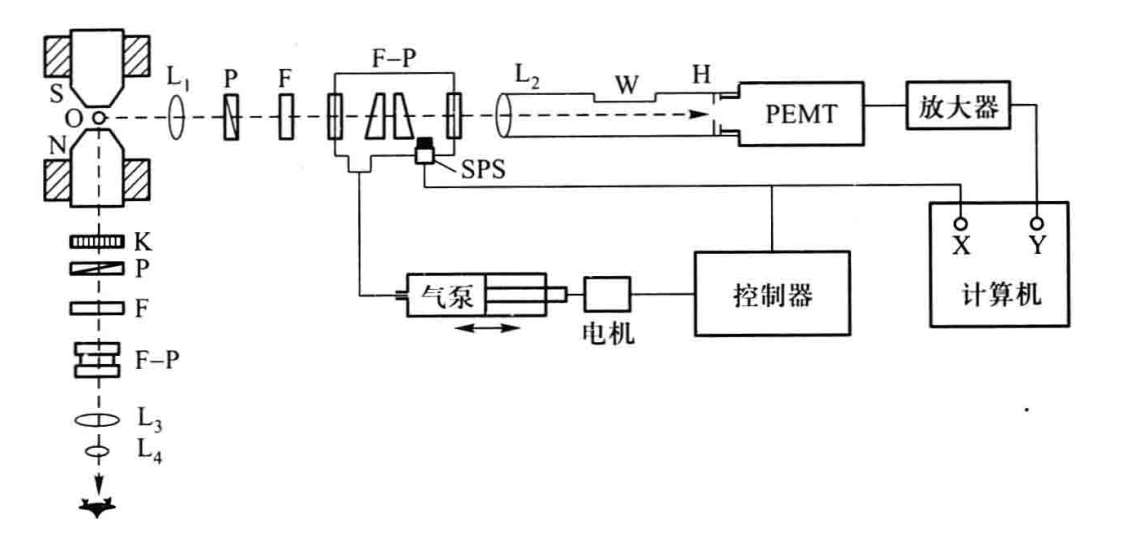
\includegraphics[width=0.85\linewidth]{fig/shiyanzhuangzhi.png}
  \caption{塞曼效应实验装置示意图}
  \label{fig:zhaungzhi}
\end{figure}


\subsection{实验步骤}
  \begin{enumerate}
    \item 开启所有仪器电源.
    \item 打开汞灯, 确定汞灯位于磁场的几何位置中心. 移动装置使得支架对准汞灯出光方向. 加上透镜装置, 使用纸屏确认透镜发出的光为平行光. 锁上毛玻璃片, 移动支架使得在毛玻璃片上呈现清晰的的像. 
    \item 粗调. 加装毛玻璃, 让眼睛分别朝三个方向移动观察, 若视线移向某一方向时, 
    中心出现 "吐出圆环" 现象, 就通过压紧该方向的旋钮或放松相反方向的旋钮来减小该方向的 h 值;若出现 "吞入圆环" 现象, 则反之. 
    反复进行这样的调节, 直至眼睛向任意方向移动时, 均不再出现上述  "吞吐现象" . 
    \item 细调. 加上针孔光阑, 调整准直. 打开气泵, 用4档升压, 如果看到有多条条纹向某个方向移动, 则把这个方向的旋钮放松或者把
相反方向的旋钮压紧 (以增大这个方向的 h) .反复调节直到升压时条纹均不向特定方向移动为止. 
    \item 测量光谱. 取下针孔光阑, 将光电倍增管套入 H 出射口并锁紧, 拔出光电倍增管一侧的开关, 可以从窗口 W 看到管中央有小灯亮起. 根据小灯和它反射光的位置调整准直. 
并看到汞灯等倾干涉环圆心和针孔光阑重合. 关闭窗口 W . 调节励磁电流分别为 0 、4 A 、5 A, 调整信号源的起始电压和量程在合适的范围, 点击电脑软件中的开始实验, 记录光谱. 
    \item 复位. 升压结束后仪器会自动停止, 此时需要点击 "复位" 按键, 并且拧松气泵的放气螺丝直至气压显示在90 mV左右后再拧紧螺丝. 
    \item 实验中需要依次测量无磁场作用, 0.8 T磁场 (4 A 励磁电流) , 1 T 磁场 (5 A 励磁电流) 的汞灯 546.1 nm 的光谱图, 并测量在 1.0 T 磁场作
用下, 汞灯$\pi$ 线和 $\sigma$ 线的光谱图.
  \end{enumerate}

\section{结果及讨论}

\subsection{实验结果}

\begin{figure}[htbp]
  \centering
  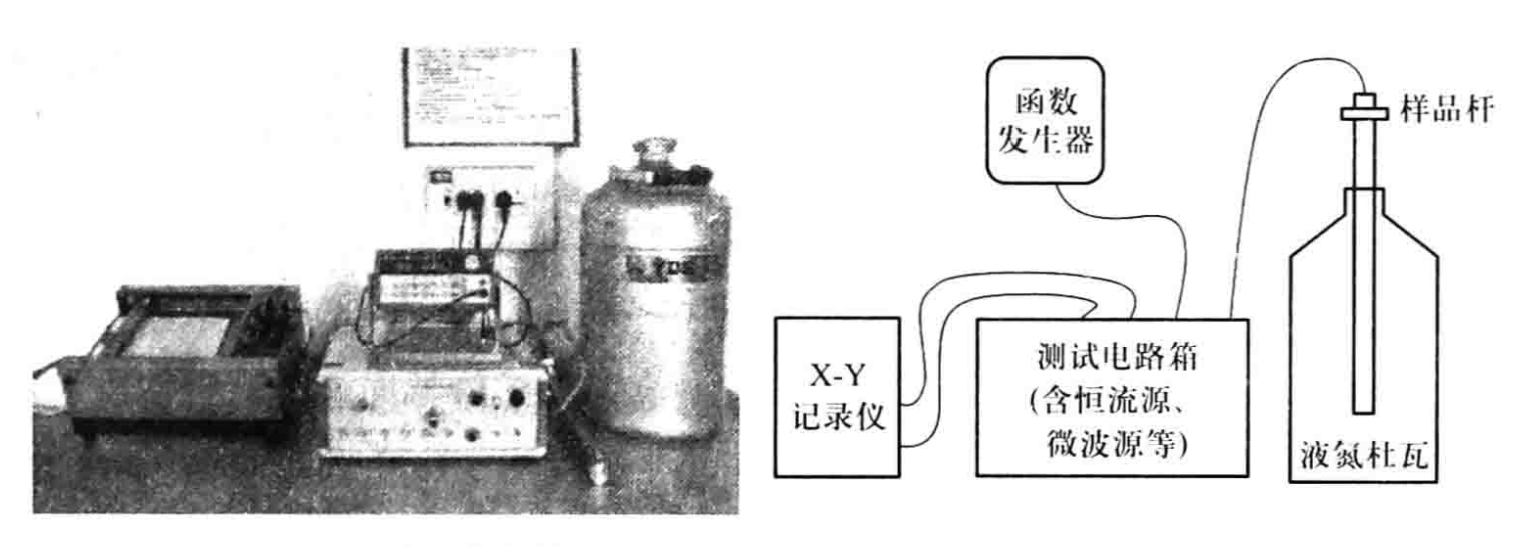
\includegraphics[width=0.85\linewidth]{fig/1.png}
  \caption{无磁场下汞灯的光谱}
  \label{fig:000}
\end{figure}

\begin{figure}[htbp]
  \centering
  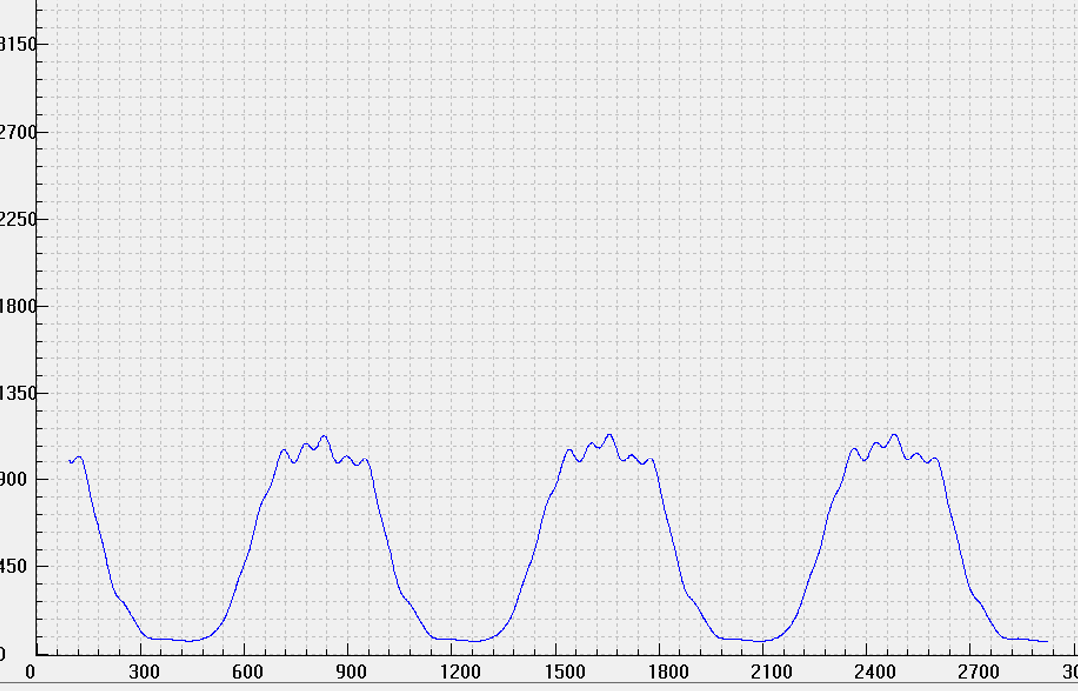
\includegraphics[width=0.85\linewidth]{fig/5.png}
  \caption{磁场为 0.8 T (I = 4 A) 下汞灯的光谱}
  \label{fig:444}
\end{figure}

\begin{figure}[htbp]
  \centering
  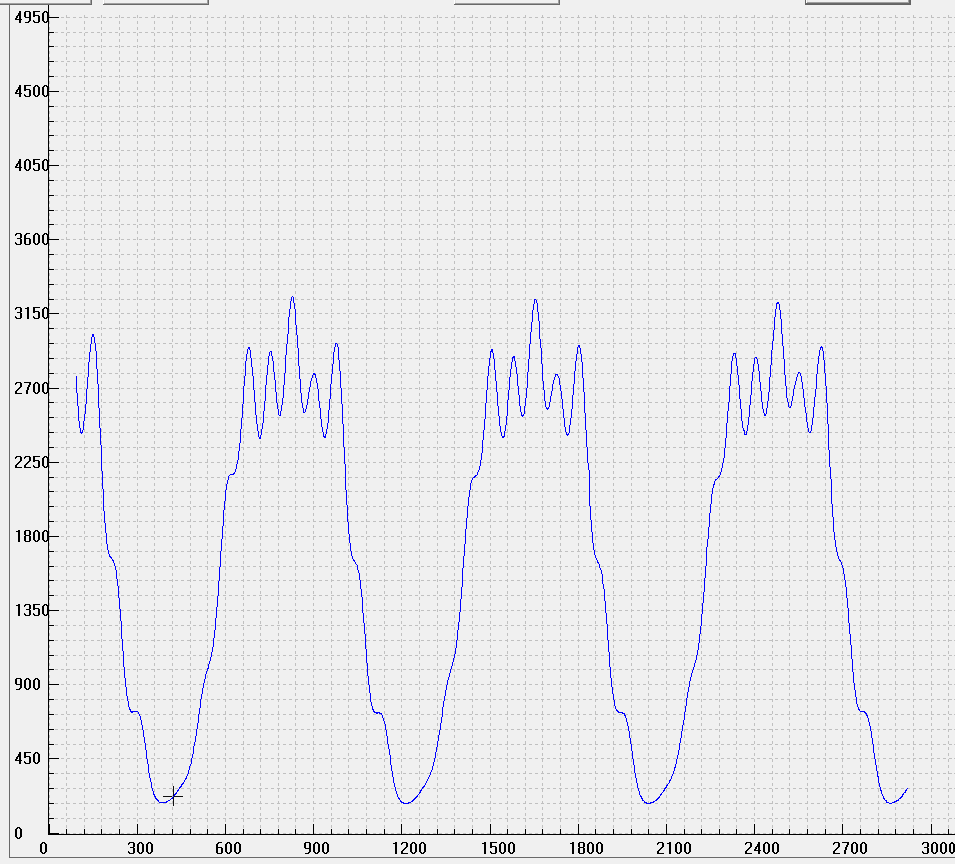
\includegraphics[width=0.85\linewidth]{fig/2.png}
  \caption{磁场为 1.0 T (I = 5 A) 下汞灯的光谱}
  \label{fig:555}
\end{figure}

  无磁场 (I = 0 A) 下汞灯的光谱如\autoref{fig:000}所示. 在一个光谱周期内, 仅存在一个 546.1 nm 的主峰. 其余的少量突起可能是精细结构的体现.
  \par
  磁场为 0.8 T (I = 4 A) 下汞灯的子谱线如\autoref{fig:444}所示, 磁场为 1.0 T (I = 5 A) 下汞灯的子谱线如\autoref{fig:555}所示. 
  相对于\autoref{fig:000}来说, 加磁场后谱线发生了分裂, 在一个光谱周期内原来的 546.1 nm 线分裂成了 9 条子谱线, 
  并且电流越大, 磁场越大, 谱线分裂得越明显. 

  在光路中加入偏振片, 旋转偏振片的角度, 在两个相互垂直的方向可以测得 $\pi$ 线和 $\sigma$ 线, 分别如\autoref{fig:551}和\autoref{fig:552}所示.
  可以看到, \autoref{fig:551}中在一个周期保留的三条线是 \pi 线, 
  而\autoref{fig:552}中在一个周期保留的六条线是\sigma线, 这和我们的理论分析\autoref{fig:lilun}一致.
  图中的杂峰没能被滤去可能是由于偏振片方向放置放的不够正确导致的.

\begin{figure}[htbp]
  \centering
  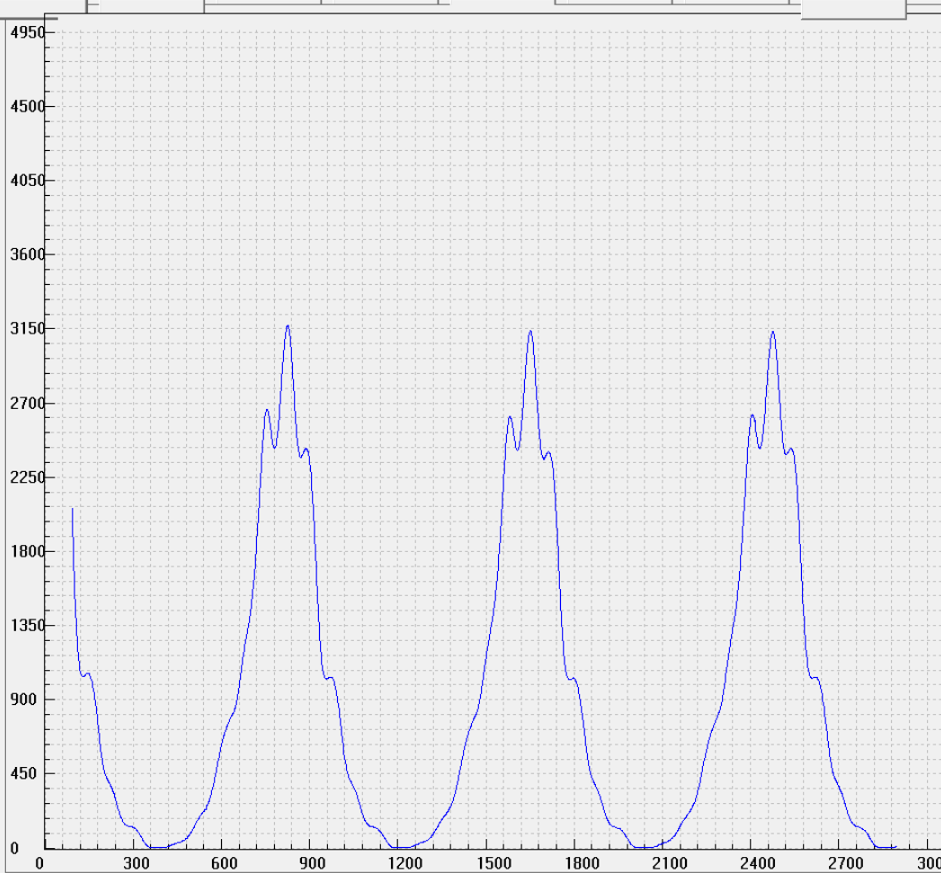
\includegraphics[width=0.85\linewidth]{fig/3.png}
  \caption{磁场为 1.0 T (I = 5 A) 下汞灯的 \pi 线}
  \label{fig:551}
\end{figure}
\begin{figure}[htbp]
  \centering
  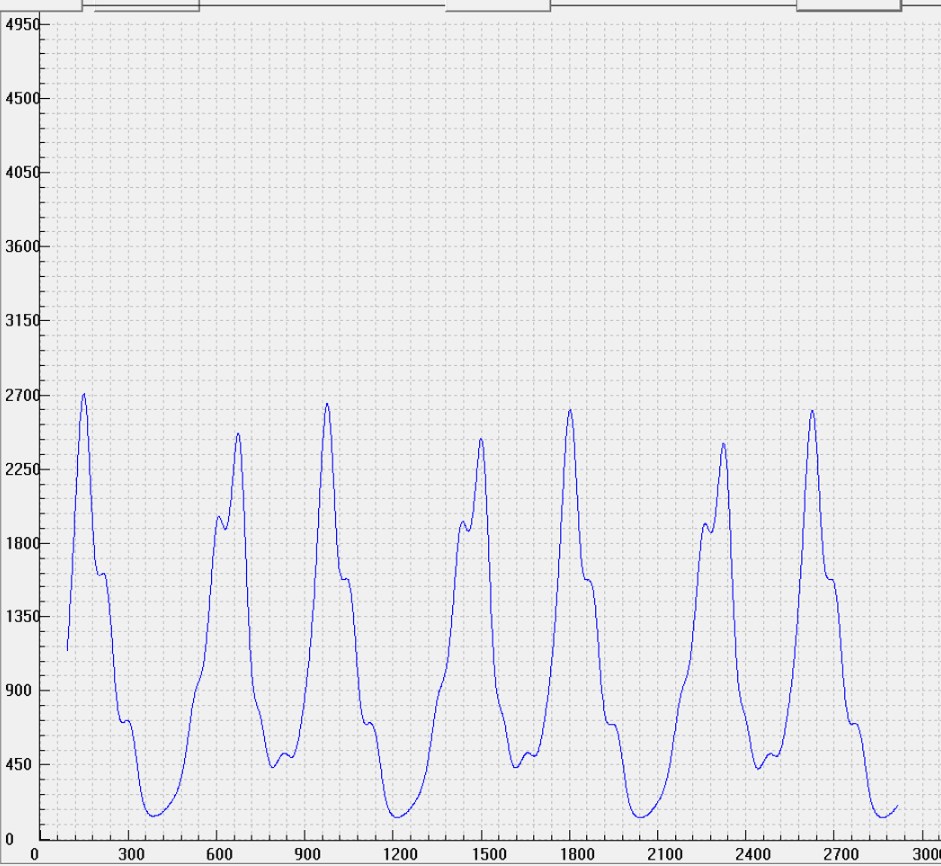
\includegraphics[width=0.85\linewidth]{fig/4.png}
  \caption{磁场为 1.0 T (I = 5 A) 下汞灯的 \sigma 线}
  \label{fig:552}
\end{figure}

\subsection{各子谱线的波数差偏移和强度}

在\autoref{fig:555}中, 分裂谱线相对于主谱线的裂距和相对强度列表分别如\autoref{tab:liejv}和\autoref{tab:qiangdu}所示
通过实验数据可以计算得出, 对于波数差$\delta \nu_R = 2.5 cm^{-1}$, 对应的压强差为 825.25 arb.units.


\begin{table}[htbp]
  \centering
  \caption{外磁场为 1.0 T 情形下, 各子谱线相对于 546.1 nm 谱线的波数差偏移}
  \begin{tabular}{c|ccccccccc}
    \hline
    n 峰 & -4 & -3 & -2 & -1 & 0 & 1 & 2 & 3 & 4 \\
    \hline
    $\Delta p$ & -284.667 & -211.667 & -148.333 & -74 & 0 & 73 & 148.667 & 216.333 & 290.333 \\
    \hline
    $\Delta \nu_{\text{exp}} (cm^{-1})$ & -0.862 & -0.641 & -0.449 & -0.224 & 0 & 0.221 & 0.450 & 0.655 & 0.880 \\
    \hline
    $\Delta \nu_{\text{theo}} (cm^{-1})$ & -0.934 & -0.701 & -0.467 & -0.234 & 0 & 0.234 & 0.467 & 0.701 & 0.934 \\
    \hline
  \end{tabular}
  \label{tab:liejv}
\end{table}

\begin{table}[htbp]
  \centering
  \caption{各子谱线的强度对比}
  \begin{tabular}{c|ccccccccc}
    \hline
    n 峰 & -4 & -3 & -2 & -1 & 0 & 1 & 2 & 3 & 4 \\
    \hline
    绝对强度 & 1012.667 & 2157.333 & 2930.667 & 2901.333 & 3237.333 & 2788 & 2961.333 & 1635.333 & 733.333 \\
    \hline
    相对强度 & 1.251 & 2.666 & 3.621 & 3.585 & 4 & 3.445 & 3.659 & 2.021 & 0.906 \\
    \hline
    相对强度理 & 0.500 & 1.500 & 3 & 3 & 4 & 3 & 3 & 1.500 & 0.500 \\
    \hline
  \end{tabular}
  \label{tab:qiangdu}
\end{table}

根据\autoref{tab:liejv}可以发现, 外磁场为 1.0 T 情形下, 
实验测得的各子谱线相对于 546.1 nm 谱线的波数差偏移与理论值比较符合, 不过所有的实验得到的波数差偏移绝对值均小于理论值.
造成这一现象的可能原因有:
\begin{itemize}
  \item 洛伦兹单位$\tilde{L} = \frac{eB}{4\pi mc} \approx 0.467B$, 但实验实际的磁场大小比理论的 1.0 T 要小.
  \item 原子内部精细结构的影响.
\end{itemize}

而分析\autoref{tab:qiangdu}会发现, 实验测得的相对强度比理论得到的大许多, 并且强度呈现左右不对称的情况. 
在左侧编号为 -4 和 -3 的峰的高度比与其对称的右侧编号为 4 和 3 的峰的高度要高很多.
造成这一现象的可能原因有:
\begin{itemize}
  \item 精细结构的影响.
  \item 实验过程中磁场与成像设备和标准具所在的直线并不垂直. 因此测量得到的谱线分裂情况并不具有各向同性, 也因此强度不对称.
  \item 分裂得到的子谱线之间挨得很近, 彼此之间会产生影响, 导致测量得到的谱线强度并不是真实的谱线强度.
\end{itemize}

\subsection{荷质比的计算}

洛伦兹单位的表达式是$$ \tilde{L} = \frac{eB}{4\pi mc}$$
从而可以得到荷质比的表达式$$\frac{e}{m} = \frac{4\pi c \tilde{L}}{B}$$

洛伦兹单位 L 的值可以由线性拟合算出. 根据\autoref{tab:liejv}的峰的变好和裂距的实验测得值, 得到如\autoref{222}所示的直线.
\begin{figure}[htbp]
  \centering
  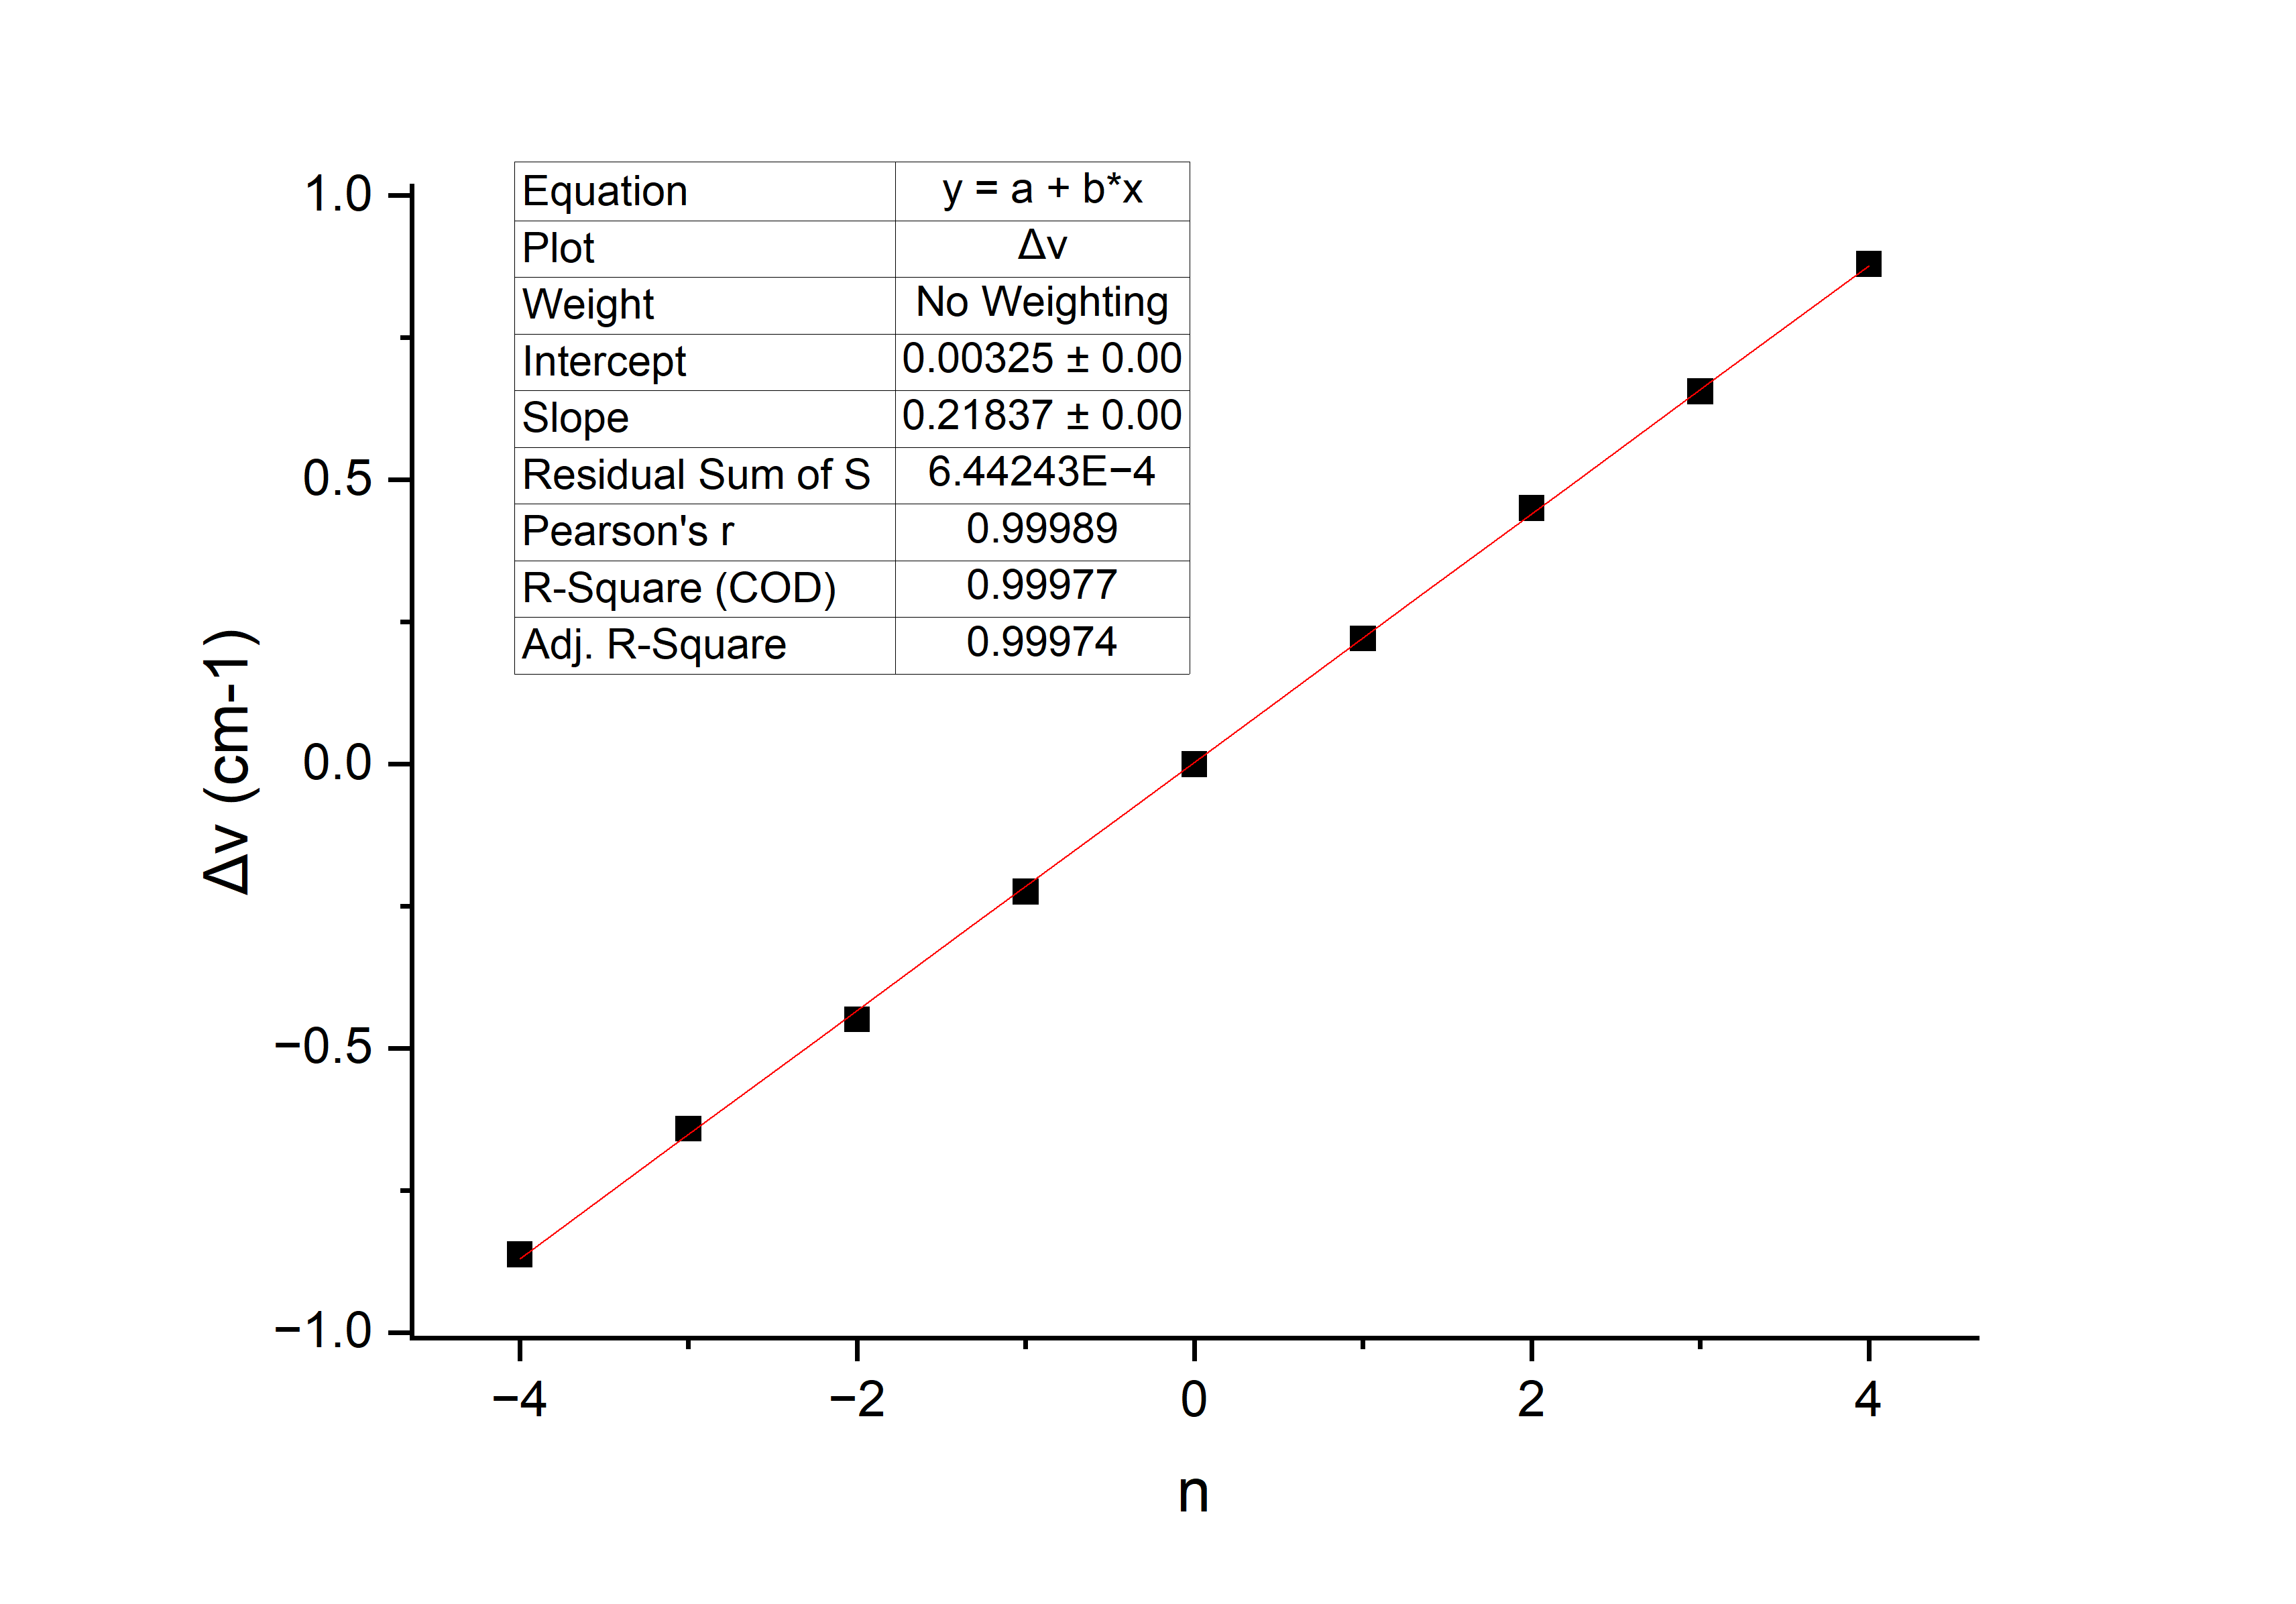
\includegraphics[width=0.85\linewidth]{fig/222.png}
  \caption{\delta \nu 与 n 的关系}
  \label{fig:222}
\end{figure}

拟合得到的斜率$$k = 0.21837 cm^{-1}$$
于是可以计算得到$$ \tilde{L} = 2k = 0.43674 cm^{-1}$$
带入磁场的大小 B = 1.0 T, 从而可以计算得到荷质比为$$\frac{e}{m} = \frac{4\pi c \tilde{L}}{B} = 1.65 \times 10^{11} C/kg$$
而查资料可知, 电子的比荷为$1.76 \times 10^{11} C/kg$, 相对误差为$ 6.25\%$. 这里误差产生的可能原因有:
\begin{itemize}
  \item 实验中实际的磁场大小不等于 1.0 T, 导致带入荷质比表达式中的 B 不准确.
  \item 在之前的讨论中有发现, 实验测得的峰与峰之间的裂距普遍比理论值小, 这会导致拟合得到的斜率偏小, 从而导致洛伦兹单位偏小, 从而使得计算得到的荷质比偏小.
\end{itemize}

 
\section{结论}
  本实验借助气压扫描式 F-P 标准具, 
  对汞灯 546.1 nm 谱线及其在磁场作用下的塞曼光谱进行观察与测量.
  报告呈现了该谱线在无磁场、0.8 T 磁场 (4 A 励磁电流) 及 1.0 T 磁场 (5 A 励磁电流) 下的光谱图, 
  同时得到了 1.0 T 磁场中 \pi 线和 \sigma 线的光谱. 
  本研究确定了 1.0 T磁场下各子谱线相对于 546.1 nm 谱线的波数差及相对强度, 
  并通过列表与理论值对比, 讨论了产生误差的原因.
  此外, 本研究还对各子谱线波数差进行拟合计算, 得到电子荷质比实验值$1.65 \times 10^{11} C/kg$, 并将其和理论值相比较, 分析了误差产生的原因.

\begin{acknowledgments}
  感谢洪浩老师和助教老师的耐心指导和帮助.
  \par
  感谢搭档王尉丞同学的协助.
\end{acknowledgments}

% bibliography 的参数是你的 *.bib 文件去掉后缀名后的部分
\bibliography{bibli}

\clearpage % 附录前另起一页
\appendix % 附录开始
\section{思考题}\label{app:exercise}
\subsection{从塞曼分裂谱中如何确定能级的 J 量子数?}
要确定能级的 $J$ 量子数, 可以利用塞曼分裂中 $\pi$ 线与 $\sigma$ 线的数目进行推断, 其逻辑如下:
首先, $\pi$ 线对应磁量子数满足 $\Delta M_J = 0$ 的跃迁. 
观测到的 $\pi$ 线数量反映了上下两个能级间相同磁量子数取值的重合情况. 
举例来说, 若出现 3 条 $\pi$ 线, 说明两个能级中有 3 个相同的磁量子数 (如 $M_J = -1, 0, 1$) . 
其次, $\sigma$ 线对应 $\Delta M_J = \pm 1$ 的跃迁. 
观测到 6 条 $\sigma$ 线, 意味着其中一个能级的磁量子数可取值为 $M_J = -2, -1, 0, 1, 2$, 即比另一个能级多出两个取值. 
结合 $\pi$ 线和 $\sigma$ 线的数目, 
可以推断出两个能级的总角动量量子数分别为 $J = 1$ 和 $J = 2$. 
\subsection{根据塞曼分裂谱的裂距如何确定能级的 g 因子数?}
根据公式$\Delta \widetilde{\nu} = (M_2 g_2 - M_1 g_1) \frac{eB}{4\pi m c} = (M_2 g_2 - M_1 g_1) \widetilde{L}$并结合各个谱线的裂距, 
可以知道各个子谱线的波数差 (即裂距) 和朗德因子 g1, g2 的关系, 可以通过实验测量得到的波数差列方程求解即可计算出两个能级的朗德因子.





\end{document}
